\subsubsection{SearchBar Component}
Το πρώτο Component μέσα στο MIDashboard Component είναι η γραμμή αναζήτησης, MISearchBar Component. Το MISearchBar Component δεν προσφέρει την δυνατότητα γενικής αναζήτησης αλλά μόνο την δυνατότητα επιλογής ενός αποτελέσματος από τις προτάσεις της μηχανής αναζήτησης. Οι προτάσεις δημιουργούνται από την μηχανή αναζήτησης μέσο του Server όπως προαναφέρθηκε νωρίτερα κάθε φορά που ο χρήστης γράφει οποιοδήποτε γράμμα στην μπάρα αναζήτησης όπως φαίνεται στον κώδικα \ref{code:searchbar_suggestion}.

\begin{figure}[H]
    \begin{TypeScriptcode}
async function getSuggestions(value: string): Promise<ACResult[]> {
    const results: AutoComplete = (await Service.search(value)).data;
    return results._
      .map(result => {
        result.e.forEach(e => {
          e.i = result.i
        })
        return result;
      })
      .filter(result => result.e.length > 0);
}
    \end{TypeScriptcode}
    \caption{Αλγόριθμος ανάκτησης προτάσεων αποτελεσμάτων μηχανής αναζήτησης}
   \label{code:searchbar_suggestion}
\end{figure}

Οι προτάσεις της μηχανής αναζήτησης εμφανίζονται με μια μικρή εικόνα στα αριστερά και το κείμενο του αποτελέσματος ακριβώς από διπλά. Ανάλογα με το κείμενο της αναζήτησης που έγραψε ο χρήστης προσπαθεί να υπογραμμίσει με μπλε χρώμα τα γράμματα που βρέθηκαν στα αποτελέσματα όπως φαίνεται στην εικόνα \ref{layout:misearchbar}.
\begin{figure}[H]
  \centering
  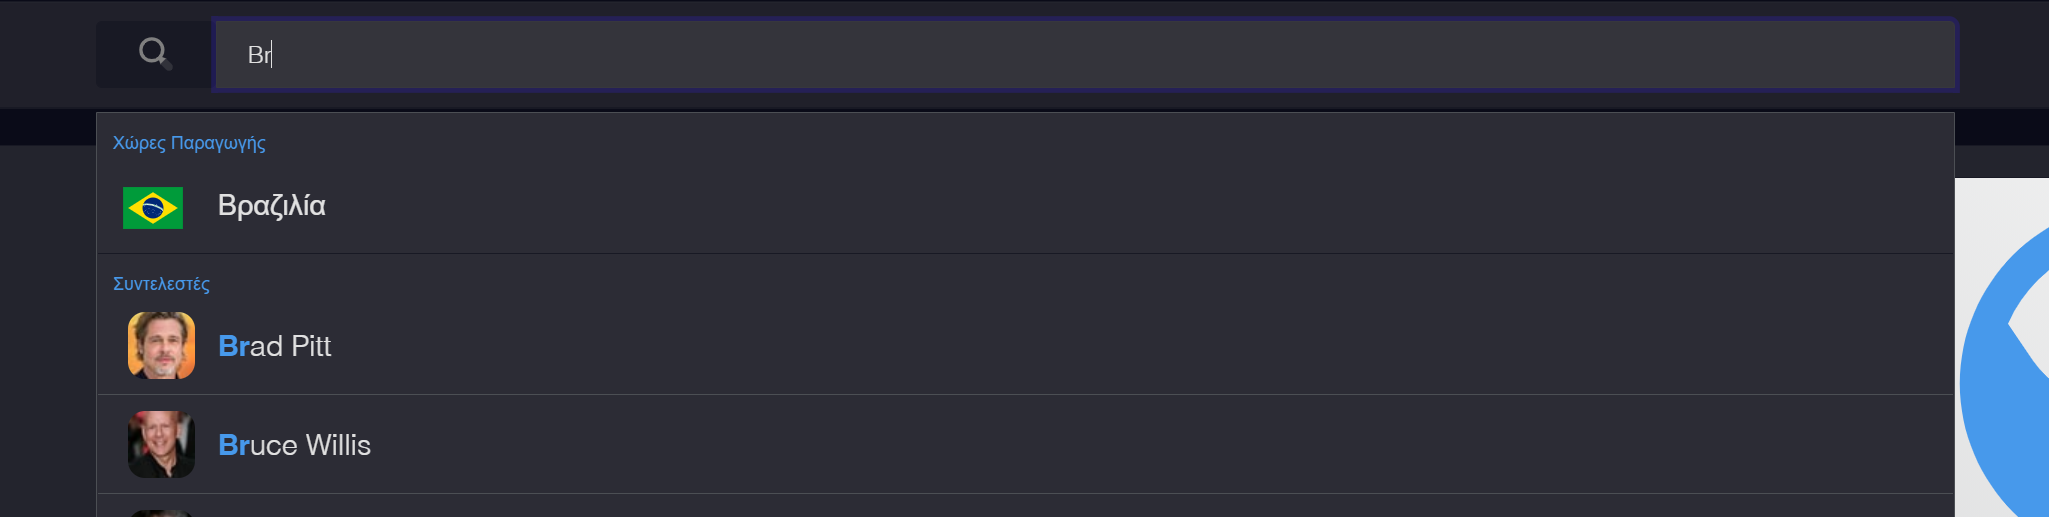
\includegraphics[width=145mm]{Chapters/5 - Architecture/Client/Images/misearchbar_results.png}
  \caption{MISearchBar Component}
  \label{layout:misearchbar}
\end{figure}
Όταν επιλεγεί ένα από τα προτεινόμενα αποτελέσματα η μπάρα αναζήτησης σβήνει και αλλάζει η διεύθυνση όπως φαίνεται στον κώδικα \ref{code:searchbar_urlchange}

\begin{figure}[H]
    \begin{TypeScriptcode}
private onSearch = (val: ACEntity) => {
  this.props.history.push(AppUtils.|\textbf{generateNavigationLink}|(val, null, null, val.i));
}
    \end{TypeScriptcode}
    \caption{Αλγόριθμος αλλαγής διεύθυνσης απο το MISearchBar Component}
   \label{code:searchbar_urlchange}
\end{figure}
